\documentclass[12pt, letterpaper]{article}
\usepackage{amsmath,amssymb,amsthm,amsopn,amscd}
\usepackage{mathtools}
\usepackage{latexsym}
\usepackage{graphicx,caption,subcaption}
\usepackage{multirow}
\usepackage[reftex]{theoremref}
\usepackage{hyperref}
\usepackage{verbatim}
\usepackage{color}
\usepackage{algorithm}      % pseudo-code
\usepackage{algpseudocode}  %
\usepackage{stmaryrd}       % double brackets
\usepackage{amstext}    % \text macro
\usepackage{array}      % \newcolumntype macro
\usepackage{tikz}       % for flow chart
\usetikzlibrary{cd}     % commutative diagram
\usetikzlibrary{shapes.geometric} % pentagon
\usepackage{graphics, tkz-berge} % icosahedron
\usepackage{afterpage}
\usepackage[export]{adjustbox}
\usepackage{tensor}
\usepackage{braket}
\usepackage{etoolbox}
\usepackage{xparse}
%   \usepackage{commath}    % for abs and norm

\usepackage{ytableau}
\usepackage{tkz-euclide}

%\setcounter{secnumdepth}{-2} % remove section numbering
\setcounter{section}{-1}

%\newcommand{\executeiffilenewer}[3]{%
%	\ifnum\pdfstrcmp{\pdffilemoddate{#1}}%
%	{\pdffilemoddate{#2}}>0%
%	{\immediate\write18{#3}}\fi%
%}
%\newcommand{\includesvg}[1]{%
%	\executeiffilenewer{#1.svg}{#1.pdf}%
%	{inkscape -z -D --file=#1.svg %
%		--export-pdf=#1.pdf --export-latex}%
%	\input{#1.pdf_tex}%
%}



\graphicspath{ {./} }

\makeatletter
\renewcommand\subparagraph{\@startsection{subparagraph}{5}{\parindent}%
	{3.25ex \@plus1ex \@minus .2ex}%
	{0.75ex plus 0.1ex}% space after heading
	{\normalfont\normalsize\bfseries}}
\makeatother

\newcommand\independent{\protect\mathpalette{\protect\independenT}{\perp}}
\def\independenT#1#2{\mathrel{\rlap{$#1#2$}\mkern2mu{#1#2}}}
\newcommand{\rp}{\mathbb{RP}}

%   Sets
\newcommand{\nat}{\mathbb{N}}
\newcommand{\inte}{\mathbb{Z}}
\newcommand{\rat}{\mathbb{Q}}
\newcommand{\re}{\mathbb{R}}
\newcommand{\renn}{\mathbb{R}_0^+}
\newcommand{\co}{\mathbb{C}}
\newcommand{\hil}{\mathbb{H}}
\newcommand{\ee}{\mathrm{e}}
\newcommand{\dd}{\mathrm{d}}
\newcommand{\GL}{\operatorname{GL}}
\newcommand{\SL}{\operatorname{SL}}
\newcommand{\PGL}{\operatorname{PGL}}
\newcommand{\PSL}{\operatorname{PSL}}
\newcommand{\MM}{\operatorname{M}}
\newcommand{\ZZ}{\operatorname{Z}}
\newcommand{\SZ}{\operatorname{SZ}}
\newcommand{\ob}{\operatorname{ob}}
\newcommand{\dom}{\operatorname{dom}}
\newcommand{\cod}{\operatorname{cod}}
\newcommand{\Hom}{\operatorname{Hom}}
\newcommand{\End}{\operatorname{End}}
\newcommand{\class}{\operatorname{class}}
\newcommand{\supp}{\operatorname{supp}}
\newcommand{\idt}{\operatorname{id}}
\newcommand{\sgn}{\operatorname{sgn}}
\newcommand{\Sym}{\operatorname{Sym}}
\newcommand{\Tr}{\operatorname{Tr}}
\newcommand{\Cl}{\operatorname{Cl}}
\newcommand{\Res}{\operatorname{Res}}
\newcommand{\Ind}{\operatorname{Ind}}

\newcommand{\ext}[1]{\bigwedge\!^{#1}}


\DeclarePairedDelimiter\ceil{\lceil}{\rceil}
\DeclarePairedDelimiter\floor{\lfloor}{\rfloor}


\newcommand{\id}{\indices}
%   \newcommand{\cp}{\mathbb{CP}}
%   \newcommand{\dS}{\mathbb{S}}
%   \newcommand{\dP}{\mathbb{P}}
%   \newcommand{\dE}{\mathbb{E}}
%   \newcommand{\dZ}{\mathbb{Z}}
\newcommand{\bfP}{\mathbf{P}}
\newcommand{\bfJ}{\mathbf{J}}
\newcommand{\bfK}{\mathbf{K}}
\newcommand{\bfR}{\mathbf{R}}
\newcommand{\idm}{\mathbf{I}}
\newcommand{\bfA}{\mathbf{A}}
\newcommand{\bfB}{\mathbf{B}}
\newcommand{\bfC}{\mathbf{C}}
\newcommand{\bfD}{\mathbf{D}}
\newcommand{\bfG}{\mathbf{G}}
\newcommand{\bfL}{\mathbf{L}}
\newcommand{\bfT}{\mathbf{T}}
\newcommand{\bfS}{\mathbf{S}}
\newcommand{\bfe}{\mathbf{e}}
%   \newcommand{\bm}{\boldsymbol{m}}
%   \newcommand{\bmu}{\boldsymbol{\mu}}
%   \newcommand{\bS}{\boldsymbol{\Sigma}}
%   \newcommand{\uvec}[1]{\mathrm{\mathbf{\hat{e}}}_#1}
%   \newcommand{\rmbf}[1]{\mathrm{\mathbf{#1}}}
%   \newcommand{\javg}{J_{\mathrm{avg^2}}}
%   \newcommand{\pgl}[1]{\mathbf{PGL}(#1,\mathbb{R})}
%   \newcommand{\Sl}[1]{\mathbf{SL}(#1,\mathbb{R})}
%   \newcommand{\gl}[1]{\mathbf{GL}(#1,\mathbb{R})}

\makeatletter
\newcommand\etc{etc\@ifnextchar.{}{.\@}}
\newcommand\ie{i.e\@ifnextchar.{}{.\@}}
\newcommand\eg{e.g\@ifnextchar.{}{.\@}}
\newcommand\Eq{Eq.\ }
\makeatother



\newcommand{\red}[1]{{\color{red} #1}}
\newcommand{\blue}[1]{{\color{blue} #1}}		

\newcommand{\power}{\mathcal{P}}
\newcommand{\domain}{\mathcal{D}}



\newcommand{\na}{\nabla}
\newcommand{\abs}[1]{\left\lvert #1 \right\rvert}
\newcommand{\card}[1]{\left\lvert #1 \right\rvert}
\newcommand{\norm}[1]{\left\lVert #1 \right\rVert}
\newcommand{\gaussian}{\mathcal{N}}
\newcommand{\define}{\coloneqq}
\newcommand{\tp}[1]{{#1}^T}
\newcommand{\hadj}[1]{{#1}^{\dagger}}
\newcommand{\conj}{\overline}
%
%   \newcommand{\lst}[2]{\{#1_{1}, #1_{2}, \dots, #1_{#2}\}}
%   \newcommand{\lstf}[2]{\{#1{1}, #1{2}, \dots, #1{#2}\}}
%   % prt stands for parenthesis
%   \newcommand{\prt}[2]{(#1_{1}, #1_{2}, \dots, #1_{#2})}
%   \newcommand{\prtf}[2]{(#1{1}, #1{2}, \dots, #1{#2})}
%   % general list formatted, #1: fxn, #2: first one, #3: last one, #4: delimiter, #5: left, #6: right
%   \newcommand{\glstf}[6]{#5 #1{#2} #4 #1{\number\numexpr#2+1\relax} #4 \dots #4 #1{#3} #6}
%
% wc = wild card
\newcommand*{\wcthin}{{\mkern 2mu\cdot\mkern 2mu}}
\newcommand*{\wc}{{}\cdot{}}    %   This one is wider
%
% Operators
% ec = equivalence class
\newcommand{\ec}[1]{\left[{#1}\right]}
% generating subgroup
\newcommand{\gensub}[1]{\left\langle{#1}\right\rangle}
%
%   automatic math mode in tabular
\newcolumntype{L}{>{$}l<{$}}
\newcolumntype{C}{>{$}c<{$}}
\newcolumntype{R}{>{$}r<{$}}

\newenvironment{centabular}{\center\tabular}{\endtabular\endcenter}
\newenvironment{centikzpic}{\center\tikzpicture}{\endtikzpicture\endcenter}
\newenvironment{centikzcd}{\center\tikzcd}{\endtikzcd\endcenter}
\newenvironment{eqlong}{\equation\aligned}{\endaligned\endequation}


\DeclareMathOperator*{\argmin}{arg\,min}
\DeclareMathOperator*{\argmax}{arg\,max}
\DeclareMathOperator{\Var}{Var}
\DeclareMathOperator{\Cov}{Cov}
\DeclareMathOperator{\rank}{rank}
\DeclareMathOperator{\spn}{span}
\DeclareMathOperator{\diag}{diag}
\DeclareMathOperator{\tr}{tr}

\newtheorem*{prop*}{Proposition}
\newtheorem{prop}{Proposition}[section]
\newtheorem*{lem*}{Lemma}
\newtheorem{lem}[prop]{Lemma}
\newtheorem{cor}[prop]{Corollary}
\newtheorem{thm}[prop]{Theorem}
\newtheorem*{thm*}{Theorem}
\newtheorem{conjec}[prop]{Conjecture}

%https://tex.stackexchange.com/questions/280313/how-to-put-the-list-of-definitions-at-contents-page
%https://tex.stackexchange.com/questions/51691/creating-list-of-for-newtheoremstyle
%\usepackage{amsthm}
%\newtheoremstyle{mystyle}
%{\topsep}{\topsep}{}{}{\bfseries}{:}{\newline}
%{\thmname{#1}\thmnumber{ #2}\thmnote{ (#3)}%
%	\ifstrempty{#3}%
%	{\addcontentsline{def}{subsection}{#1~\thedef}}%
%	{\addcontentsline{def}{subsection}{#1~\thedef~(#3)}}}
%
%\theoremstyle{mystyle}
%\newtheorem*{def*}{Definition}
\theoremstyle{definition}
\newtheorem*{defaux}{Definition}

%https://tex.stackexchange.com/questions/60872/ams-theorems-in-table-of-contents
\NewDocumentEnvironment{def*}{o}
{\IfNoValueTF{#1}
	{\defaux\addcontentsline{toc}{subsubsection}{\protect\numberline{}Definition}}
	{\defaux[#1]\addcontentsline{toc}{subsubsection}{\protect\numberline{}Definition (#1)}}%
	\ignorespaces}
{\label{#1}}
{\enddefaux}

%\makeatletter
%\newcommand\definitionname{Definition}
%\newcommand\listdefinitionname{List of Definitions}
%\newcommand\listofdefinitions{%
%	\section*{\listdefinitionname}\@starttoc{def}}
%\makeatother

\theoremstyle{remark}
\newtheorem*{rem*}{Remark}
\newtheorem*{ack*}{Acknowledgements}

\theoremstyle{definition}
\newtheorem{exe}{Exercise}[section]
\newtheorem{exe*}[exe]{Exercise*}
\newtheorem{exam}[exe]{Example in Book}
\newtheorem{eq}[exe]{Equation in Book}
\newtheorem{ddef}[exe]{Definition in Book}
\theoremstyle{plain}
\newtheorem{pprop}[exe]{Proposition in Book}
\newtheorem{ccor}[exe]{Corollary in Book}
\newtheorem{llem}[exe]{Lemma in Book}
\newtheorem{tthm}[exe]{Theorem in Book}
\captionsetup{width=0.9\textwidth}


%%  \usetikzlibrary{shadows}% for shadow
%%  \tikzstyle{event} = [color=black!40,text=white,text centered,circular drop shadow,font=\large\bfseries,text height=4em,text width=4em]
%   \tikzstyle{event} = [draw, circle]
%   \tikzstyle{arrow} = [thick,->,>=stealth]
%%  \usetikzlibrary{arrows}
%%  \tikzstyle{arrow} = [draw, -latex', thick]
%
%   %only for this doc
%   \newcommand{\llb}{\llbracket}
%   \newcommand{\rrb}{\rrbracket}

%opening
\title{Reading Notes for \\ \large \textit{Elementary Topology: Problem Textbook}}
\author{Zhi Wang}

\begin{document}
	
	\ytableausetup{centertableaux}
	
	\maketitle
	
	\tableofcontents
	\begin{def*}[arithmetic progression]
		An \textbf{arithmetic progression} or arithmetic sequence is a sequence of numbers such that the difference between the consecutive terms is constant:
		\[a_1,a_1+d,a_1+2d,\dots.\]
	\end{def*}
	
	%	\listofdefinitions
	\begin{def*}[point]
		Elements in $X$ given a topology $(X,\Omega)$ are called \textbf{points}.
	\end{def*}
	\begin{def*}[particular point topology]
		Given a discrete topology 
		\[(X,\power(X)),\]
		and a singleton $\set{a}$ disjoint with $X$,
		a \textbf{particular point topology} or \textbf{topology of everywhere dense point} is
		\[(X\cup \set{a}, \set{\set{a}\cup U|U\in\power (X)}\cup \set{\emptyset}). \]
		
	\end{def*}
	\begin{rem*}
		Let $(Y, \Omega)$ be a particular point topology,
		then
		\[S \in \Omega\iff S=\emptyset \lor a \in S,\]
		\ie, $a$ belongs to any nonempty open set.
	\end{rem*}
	\begin{def*}[Sierpiński space]
		A particular point topology with two points is called
		a \textbf{Sierpiński space} or topology of
		connected pair of points. Explicitly, it is
		\[(\set{a,b},\set{\emptyset,\set{a},\set{a,b}}), \]
		where $a\ne b$ and $a$ being the element in all nonempty open sets.
	\end{def*}

	\begin{def*}[Cantor set]
		Let $K$ be the set of real numbers that are sums of series of the form
		\[\sum_{k=1}^{\infty}
		a_k 3^{-k},\]
		with $a_k \in \set{0,2}$. In other words, $K$ is the set of real numbers
		that are presented as $0.a_1a_2 \dots a_k \dots$ without the digit 1 in the positional
		system with base 3.
		$K$ is called the \textbf{Cantor set}.
	\end{def*}
	\begin{rem*}
		Then any real number of form $x3^{-j}\in[0,1]$ ($x\in\nat,j\in\nat$) must be in $K$.
		But $K$ contains irrational numbers as well.
		\[K\cap \rat=\set{\sum_{p\in P}\frac{2\cdot3^p}{3^{i}}+\sum_{q\in Q}\frac{2\cdot3^q}{3^j-3^i}|0\le p< i\le i+q< j, }. \]
	\end{rem*}

	\begin{def*}[family]
		A \textbf{family} of a set $S$ is a subset of $\power(S)$.
		
		Equivalently, a collection $F$ of subsets of a given set $S$ is called a family of subsets of $S$, or a family of sets over $S$.
	\end{def*}
	\begin{def*}[base]
		A \textbf{base} or basis for the topology $\Omega$ of a topological space $(X, \Omega)$
		is a family $B$ of open subsets of $X$ such that every open set of the topology is equal to a union of some sub-family of $B$.
		
		Equivalently, $B$ is a base of topology $(X, \Omega)$ if
		\[S\in\Omega\iff \exists B'[B'\subseteq B\land S=\cup B'].\]
	\end{def*}
	\begin{rem*}
		Topologies on a set $X$ with only one base are exactly
		$\mathcal{S}\in\power(\power(X))$
		such that \[\set{\emptyset,X}\subseteq \mathcal{S} \land \forall \mathcal{T}\subseteq\mathcal{S}[\mathcal{T}\ne\emptyset\implies \exists
		M\in \mathcal{T}\forall T\in \mathcal{T}( T\subseteq M)],\]
		\ie, a topology whose nonempty subset $\mathcal{T}\subseteq \mathcal{S}\subseteq\power(X)$
		must have an element containing all other elements in $\mathcal{T}$.
		
		Example:
		$\re$ whose open sets are intervals $(-1/n,1/n)$ for $n\in \inte^+$, $\emptyset$, and $\re$.
		
		Example2:
		For any finite sequence $\emptyset\subseteq X_1\subseteq X_2\subseteq\dots\subseteq
		X_n\subseteq X$, the topology on $X$ consisting of those sets provides another example.
	\end{rem*}

	\begin{def*}[subbase]
		Let $(X, T)$ be a topological space.
		A \textbf{subbase} of $T$ is usually defined as a $B \subseteq T$
		satisfying one of the two following equivalent conditions:
		\begin{itemize}
			\item $T$ is the smallest topology containing $B$:
			any topology $T'$ on $X$ containing $B$ must also contain $T$.
			\item All finite intersections of elements of $B$, together with the set $X$, forms a basis for $T$, \ie,
			\[\Sigma=\set{\bigcap_{i=1}^n B_i |n\in\inte^+,B_i\in B}\cup\set{X} \]
			is a base of $T$.
		\end{itemize}

		For any $S \subseteq \power(X)$, there is a \textbf{unique} topology having $S$ as a subbase. In particular, the intersection of all topologies on $X$ containing $S$ satisfies this condition. \red{In general, however, there is no unique subbasis for a given topology. ???}
	\end{def*}

	\begin{def*}[metric space]
		See book.
	\end{def*}
	\begin{rem*}
		Consider a metric space 
		\[(X=\set{x,y,z},\rho\colon X\times X\to \re_{0}^{+}) ,\]
		where
		\[\rho(x,y)=\rho(x,z)=4,\rho(y,z)=7.
		\]
		Then \[\set{x,y}=B_6(y)\subsetneqq B_5(x)=\set{x,y,z}.\]
	\end{rem*}

	\begin{rem*}
		Given $a,b\in\re^2$, the set
		\[\set{ x \in \re^2 | \rho(a,x) + \rho(x,b) =\rho(a,b) }\]
		is the line segment if $\rho$ is the Euclidean metric.
	\end{rem*}

	\begin{center}
		
		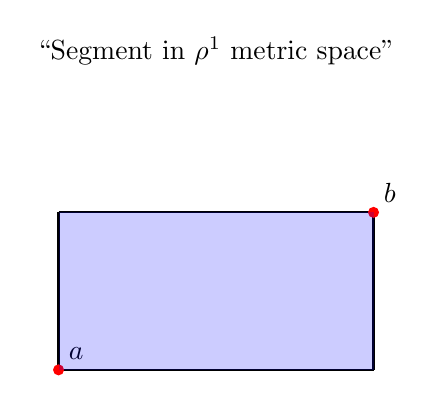
\begin{tikzpicture}
			\tkzInit[xmax=5,ymax=3,xmin=-1,ymin=-1]
			\tkzAxeXY
			\coordinate (a) at (0,0);
			\coordinate (b) at (4,2);
			\draw[ thick] (0,2) -- (0,0) node[anchor=south west] {$a$};
			\draw[ thick] (0,0) -- (4,0) ;
			\draw[ thick] (0,2) -- (4,2) node[anchor=south west] {$b$};
			\draw[ thick] (4,0) -- (4,2) ;
			\fill[red] (a) circle (2pt);
			\fill[red] (b) circle (2pt);
			\fill [draw=none, fill=blue, fill opacity=0.2] 
			(0,0) rectangle (4,2);
			\tkzText[above](2,3.75){``Segment in $\rho^1$ metric space''}
		\end{tikzpicture}
		
		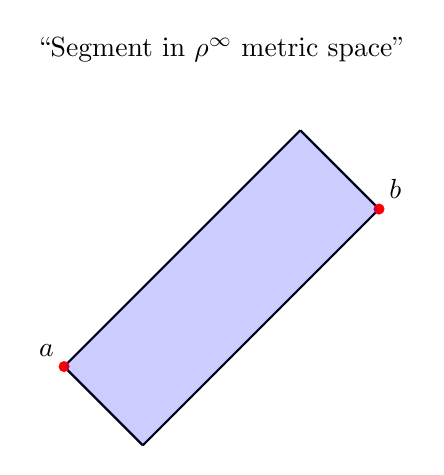
\begin{tikzpicture}
			\tkzInit[xmax=5,ymax=3,xmin=-1,ymin=-1]
			\tkzAxeXY
			\coordinate (a) at (0,0);
			\coordinate (b) at (4,2);
			\draw[ thick] (3,3) -- (0,0) node[anchor=south east] {$a$};
			\draw[ thick] (0,0) -- (1,-1) ;
			\draw[ thick] (3,3) -- (4,2) node[anchor=south west] {$b$};
			\draw[ thick] (1,-1) -- (4,2) ;
			\fill[red] (a) circle (2pt);
			\fill[red] (b) circle (2pt);
			\fill [draw=none,rotate=45, fill=blue, fill opacity=0.2] 
			(0,0) rectangle ({3*sqrt(2)},{-sqrt(2)})
			;
			\tkzText[above](2,3.75){``Segment in $\rho^\infty$ metric space''}
		\end{tikzpicture}
	\end{center}

	\begin{def*}[dense]
		Let $A$ and $B$ be two sets in a topological space $X$.
		$A$ is \textbf{dense} in $B$ if $B$ is a subset of the closure of $A$.
		$A$ is \textbf{everywhere dense} if the closure of $A$ is $X$.
		A set is \textbf{nowhere dense} if its exterior is everywhere dense.
	\end{def*}
	\begin{thm*}
		A set is everywhere dense iff it intersects any nonempty open set.
	\end{thm*}
	\begin{thm*}
		A set is nowhere dense iff its closure has empty interior.
	\end{thm*}

	\begin{def*}[limit point]
		A point $b$ is a \textbf{limit point} of a set $A$,
		if each neighborhood of $b$ intersects
		$A \setminus \set{b}$.
	\end{def*}
	\begin{thm*}
		Every limit point of a set is its adherent point.
		The reverse is not true.
	\end{thm*}
	\begin{thm*}
		A set is closed iff it contains all of its limit points.
	\end{thm*}
	\begin{def*}[isolated point]
		A point $b$ is an \textbf{isolated point} of a set $A$
		if $b \in A$ and $b$ has a neighborhood
		disjoint with
		$A \setminus \set{b}$.
	\end{def*}

	$U$ is open in $X$ iff\\
	$\forall x\in U\exists V\subseteq X$ 
	[$x\in V$ and $V$ is open $X$ and $U\cap V$ is open in $V$].
	\begin{center}
		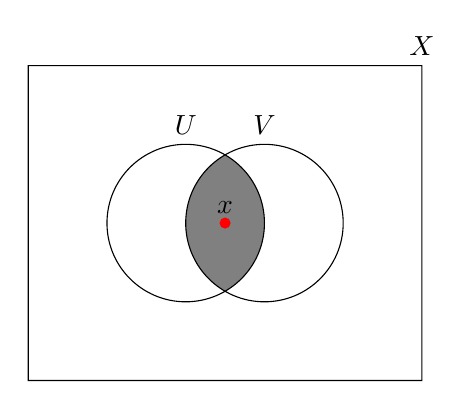
\begin{tikzpicture}[fill=gray]
			% left hand
			\scope
			\clip 
			(1,0) circle (1);
			\fill (0,0) circle (1);
			\endscope
			% right hand
			\scope
			\clip (-2,-2) rectangle (2,2)
			(0,0) circle (1);
			%\fill (1,0) circle (1);
			\endscope
			% outline
			\draw (0,0) circle (1) (0,1)  node [text=black,above] {$U$}
			(1,0) circle (1) (1,1)  node [text=black,above] {$V$}
			(-2,-2) rectangle (3,2) node [text=black,above] {$X$};
			\fill[red] (0.5,0) circle (2pt) node [text=black,above] {$x$};
		\end{tikzpicture}
	\end{center}
	
	Therefore we can say $U$ is locally open:
	a set $U$ is open iff it is open in a neighborhood $V$ of each of
	its points.
	\begin{center}
		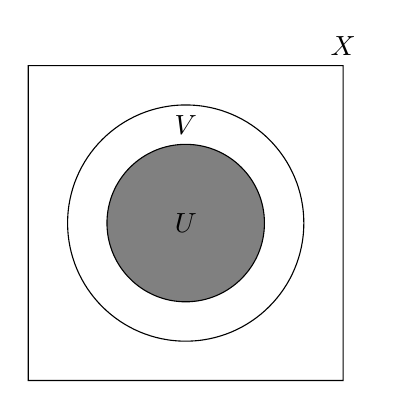
\begin{tikzpicture}[fill=gray]
			\fill (0,0) circle (1);
			\draw (0,0) circle (1) (0,0)  node [text=black] {$U$}
			(0,0) circle (1.5) (0,1.0)  node [text=black,above] {$V$}
			(-2,-2) rectangle (2,2) node [text=black,above] {$X$};
		\end{tikzpicture}
	\end{center}

	But a locally closed set is not closed.
	\begin{def*}[locally closed set]
		Given a topology $(X,\Omega)$, below are equivalent statements
		\begin{itemize}
			\item $A$ is \textbf{locally closed} in $X$;
			\item $A$ is an open subset of its closure;
			\item $A$ is the intersection of open and closed subsets of $X$;
			\item $A$ is closed in the subspace $(U,\Omega_U)$,
			where $U$ is an open set containing $A$,
			\ie, $U\in\Omega \land A\subseteq U$.
		\end{itemize}
	\end{def*}

	
	\begin{def*}[smallest neighborhood space]
		A space satisfying one of the below conditions is a \textbf{smallest neighborhood space}.
		
		The following statements are equivalent
		\begin{itemize}
			\item each point has a smallest neighborhood,
			\item the intersection of any collection of open sets is open,
			\item the union of any collection of closed sets is closed.
		\end{itemize}
	\end{def*}
	\begin{def*}[Khalimsky line]
		The poset topology on $\inte$ with the base
		\[ \set{\set{2k-1,2k,2k+1}|k\in\inte}  \]
		is called
		the \textbf{digital line}, or \textbf{Khalimsky line}.
	\end{def*}
	\begin{thm*}
		In the digital line,
		each even number is closed and each odd one is open.
	\end{thm*}
	\begin{def*}[cyclic order]
		A finite cyclic group naturally defines a \textbf{cyclic order}.
	\end{def*}

	The cyclic order topology determined by the cyclic counterclockwise
	order of $S^1$
	is the topology generated by the metric $\rho(x,y) = \abs{x - y}$ on
	$S^1 \subseteq\co$.
	
	\begin{def*}[locally continuous]
		A map $f$ from a topological space $X$ to a topological space $Y$ is said to
		be \textbf{continuous at a point} $a \in X$ if for every neighborhood $V$ of $f(a)$ there
		exists a neighborhood $U$ of a such that $f(U) \subseteq V$.
	\end{def*}

	\red{p60 isometric embedding, isometry and after skipped}
	
	
\end{document}
